\Exercise[number={6}]
A variable \(x\) in \(\mathbf{R}^2\) is emitted by three possible sources,
\(w_1\), \(w_2\), \(w_3\) of probability \(Pr(w_1)=Pr(w_2)=Pr(w_3)\). 
All three \(p(x|w_i)\) have a Gaussian distribution, with
mean \(\mu_i\) and equal variances \(I\sigma^2\). We want to design a Bayes
classifier, which assigns the correct class to each observed \(x\).
Prove that the decision regions are delimited by the axes of the sides of the
triangle with vertices \(\mu_1\),\(\mu_2\), and \(\mu_3\) and in particular
pass through the center of the circumscribed circumference of the triangle
(circumcenter).

\Answer[number={6}]
It might be useful to study the decision boundaries between the three
couples of classes \(w_1\) and \(w_2\), \(w_2\) and \(w_3\), and
finally \(w_1\) and \(w_3\).\\
Let's start by deriving the first case (\(w_1\) and \(w_2\)):
\begin{align*}
    z(x)
    &=\log{\frac{p(x|w_1)}{p(x|w_2)}} + \cancel{\log{\frac{Pr(w_1)}{Pr(w_2)}}}
    =\log{p(x|w_1)}-\log{p(x|w_2)}\\
    &=-\cancel{\log{\frac{2\pi}{2\pi}}}-\cancel{\frac{1}{2}\log{\frac{|\Sigma_1|}{|\Sigma_2|}}}-\frac{1}{2\sigma^2}\bigl[(x-\mu_1)^T(x-\mu_1)-(x-\mu_2)^T(x-\mu_2)\bigr]\\
    &=-\frac{1}{2\sigma^2}\bigl[(\mu_1^T\mu_1-\mu_2^T\mu_2)-2(\mu_1-\mu_2)^Tx\bigr]\\
    &=-\frac{1}{2\sigma^2}\bigl[(\mu_1-\mu_2)^T(\mu_1+\mu_2-2x)\bigr]\\
    &=\frac{1}{\sigma^2}\biggl[(\mu_1-\mu_2)^T(x-\frac{\mu_1-\mu_2}{2})\biggr]
\end{align*}
\begin{align*}
    z(x)=0 \Longleftrightarrow \frac{1}{\sigma^2}\biggl[(\mu_1-\mu_2)^T(x-\frac{\mu_1-\mu_2}{2})\biggr]=0
\end{align*}
Once again, the decision boundary is given by the perpendicular bisector
of segment connecting \(\mu_1\) and \(\mu_2\).
A similar computation leads to the decision boundaries for the other two
cases, still the perpendicular bisectors for the segments connecting the
centers \(\mu_i\) of the selected classes.
Now, let's exploit the superimposition principle to combine the three
distinct decision boundaries:
\begin{figure}[H]
    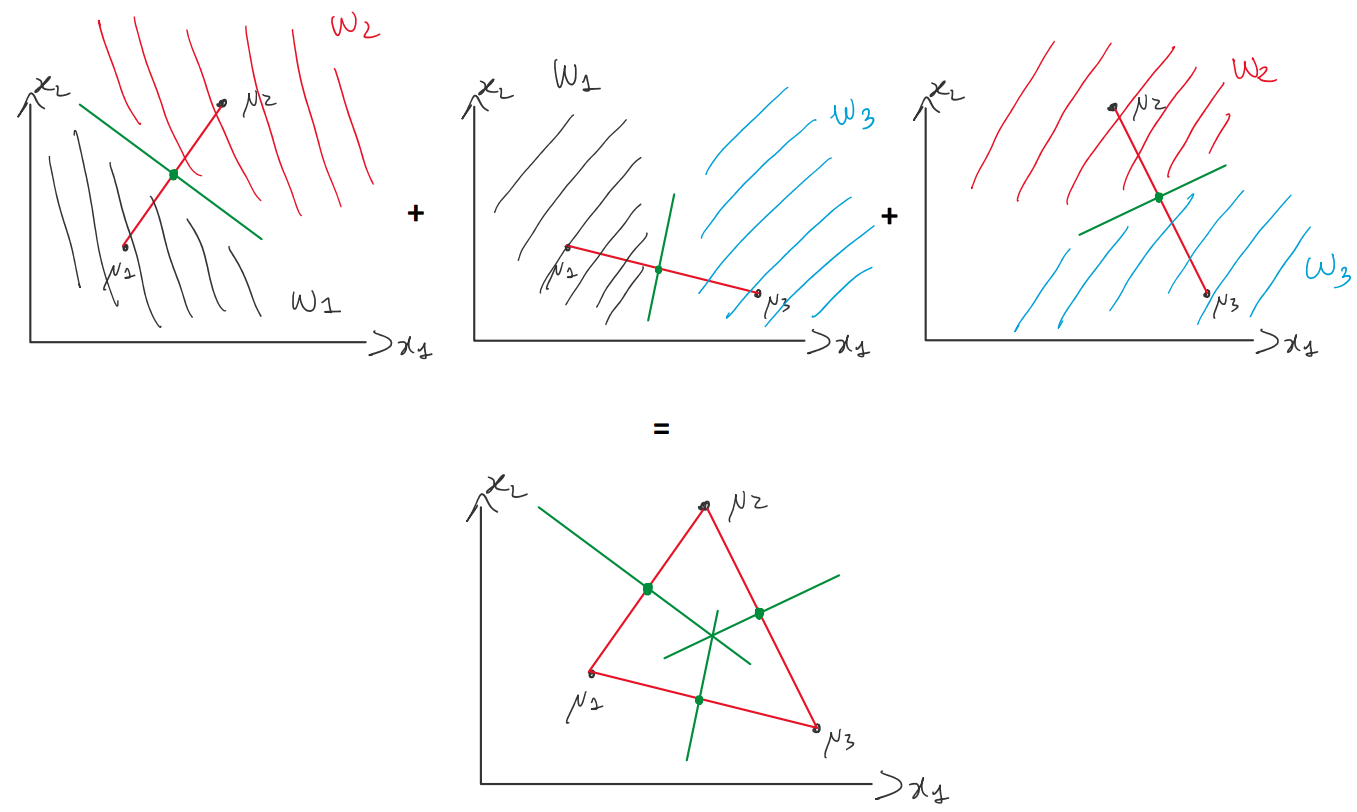
\includegraphics[scale=0.6]{C_6_1}
    \centering
\end{figure}
At this point, it is not difficult to state that the intersecting point
for the three decision boundaries must be the circumcenter for the
triangle defined by the vertices \(\mu_1\), \(\mu_2\) and \(\mu_3\),
as the three decision lines represent the perpendicular bisectors
for the triangle sides. Therefore, that point is coincident with the center
of the circumscribed circumference, by the definition of circumcenter.
\begin{figure}[H]
    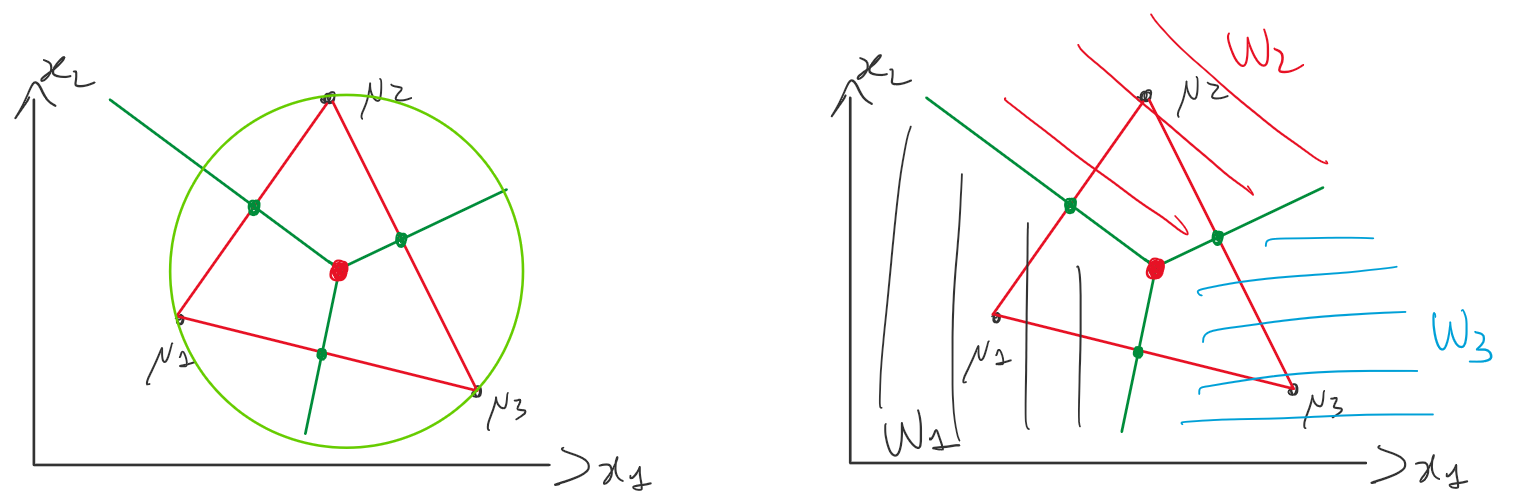
\includegraphics[scale=0.45]{C_6_2}
    \centering
\end{figure}